{
\chapter{Introduction}
\label{ch:intro}
\renewcommand{\chapterpath}{includes/intro}
Visual information plays a remarkably prominent role in how humans and many other animals perceive the world. By way of illustration, about 27 \% of the cerebral cortex of humans and 52 \% of the macaque monkey's is devoted to vision \citep{vanessen2003visualcortex}. This involves billions of neurons and connections which give rise to very complex and sophisticated mechanisms, such as visual attention and object recognition. Understanding the way visual information is processed in the brain and how it affects our behaviour is a very active area of research in cognitive science and neuroscience. In turn, developing artificial algorithms that mimic some aspects of biological vision by learning patterns from collections of image data is another active and currently fruitful area of research in machine learning and computer vision. While all these disciplines are rooted in significantly different origins and make use of distinct tools, there are grounds to defend that the interdisciplinary study of these areas of research can highly benefit each other \citep{bengio2015dlandneuroscience, marblestone2016dlandneuroscience, hassabis2017aiandneuroscience, bowers2017pdp, richards2019dlandneuroscience, kietzmann2019dnncompneuro, lindsay2020dlandneuroscience, saxe2020dlandneuroscience}.

In this thesis, we study several aspects of vision and image understanding, such as visual object recognition and visual attention, using the methods and techniques of various disciplines. In particular, we approach machine visual object recognition through deep artificial neural networks, compare some of their properties with the visual cortex, and draw inspiration from visual perception and biological vision to improve the artificial models; we employ eye tracking to analyse the global salience of images when humans look at competing stimuli; and we study the effectiveness of visual salience to identify images from fMRI data. Overall, this dissertation aims at integrating knowledge and methodologies of various disciplines to further advance our understanding of biological and artificial vision.

Summarised, the specific contributions of this thesis are the following: we shed light on the heavily understudied role of data augmentation---transformations of the input data---on training artificial neural networks for image object recognition, and show that it is more effective than the most popular regularisation techniques. Additionally, we found that models trained with heavier image transformations may learn internal representations more aligned with the activations measured in the visual cortex of the brain. Further, we demonstrate how data augmentation can be used to incorporate inductive biases---useful priors---from visual perception and biological vision, in particular the invariance to identity-preserving transformations. Separately, we propose the concept of image global salience, a property of natural images that reflects the likelihood of a stimulus to attract the gaze of a human observer when presented in competition with other stimuli. Finally, we studied the correlation of image salience with the measured activations in the visual cortex.

The interdisciplinary nature of this thesis is rooted in the breadth of my\footnote{Except in the cases where I refer explicitly to me---the author of this thesis---as an individual or intend to express my personal opinion, I will use, in general, the plural form of the first person in order to acknowledge the contribution of some collaborators to certain parts of the work and keep a consistency throughout the whole thesis.} personal interests as well as in the opportunities that the characteristics of my PhD programme offered to me. Having a background on computer science and electrical engineering, already my Bachelor's thesis \citep{hernandez2014bscthesis} addressed the problem of predicting subjective perception from audiovisual content, work continued in my Master's thesis, where I used psychophysical measurements \citep{hernandez2017mscthesis}. My journey towards cognitive science went on when I was admitted as a PhD candidate in the Institute of Cognitive Science of the University of Osnabrück, with Professor Peter König---although in practice I lived and worked in Berlin. The PhD programme also gave me the opportunity to get in touch, for the first time, with neuroscience, as I became a fellow of the Marie Skłodowska-Curie Innovative Training Network ``Training the next generation of European visual neuroscientists" (\href{http://nextgenvis.eu}{NextGenVis\footnote{\href{http://nextgenvis.eu}{www.nextgenvis.eu}}}). In spite of the challenges of being an outlier in the cohort of PhD students as a machine learning scientist, the breadth of my interests certainly expanded. As a mandatory aspect of the Marie Skłodowska-Curie grant, I had to carry out two 2-months internships at laboratories of the partnership or related. This gave me the opportunity to work at the Spinoza Centre for Neuroimaging in Amsterdam with Dr. Serge Dumoulin, where I worked on the project that is described in Chapter~\ref{ch:imageid}; and at the Cognition and Brain Sciences Unit of the University of Cambridge with Dr. Tim Kietzmann, where I started the work that yielded Chapter~\ref{ch:invariance}. I am very greateful to Serge, Tim and Peter for these opportunities.

The breadth of one's interests and work is certainly at odds with depth. However, there is probably not a single sweet spot in the trade-off between breadth and depth valid for all scientists. I understand science as a collaborative ecosystem that is most effective if scientists are distributed across the whole spectrum of the breadth-depth dichotomy. This thesis---and my work so far---is an attempt to explore the interdisciplinary approach to science, in particular to the study of learning systems---artificial and biological---specialised in visual information.

\section{Learning to see}
\label{sec:intro-learning_to_see}
Vision has evolved as one of the most advanced perceptual mechanisms in humans and many other animals, and is the main source of information for most of us to navigate and understand the world around us. Among the multiple high-level perceptual abilities achieved by our visual system, one of the most sophisticated and best studied is visual object recognition: under an enormous variety of conditions, humans can easily distinguish objects of different categories as well as identify individual objects within the same class \citep{logothetis1996objectrecognition}. Being such an important aspect of human perception, automatically finding and identifying objects from digital images has been as well an active area of research in computer vision and a technological challenge for several decades.

The task of image object recognition in computer vision can be defined in its simplest case as the categorisation of an image into one class from a set of pre-defined object classes, according to the main object present in the image by extracting and processing the visual information, that is the pixel values. Object recognition is closely related to other tasks such image object detection \citep{zhao2019objectdetection} and content-based image retrieval \citep{latif2019imageretrieval, zhou2017imageretrieval}. The generalisation of this broader set of of tasks is known as \textit{image understanding}. Ultimately, the goal of artificial image understanding is to extract rich and complex information from a digital image, as close as possible to biological vision and visual perception.

During several decades, object recognition and the related tasks of image understanding were predominantly approached by extracting handcrafted features from the images to then train machine learning classifiers. As a result, much of the computer vision literature was dominated by the proposal and refinement of image processing techniques, such as edge detectors, line and curve detectors like the Hough transform \citep{duda1972hough}, scale-invariant feature descriptors such like SIFT \citep{lowe2004sift} and HOG \citep{dalal2005hog} or Haar-like features \citep{lienhart2002haar}, among many others. These features are usually combined using bag-of-visual-words techniques \citep{sivic2003bog} to train classifiers such as support vector machines (SVM) \citep{cortes1995svm}; or more sophisticated approaches such as Fisher kernels \citep{perronnin2007fisher}. Today, these techniques are informally known as \textit{traditional} machine learning or \textit{traditional} computer vision.

What currently is considered \textit{modern} machine learning are \textit{deep artificial neural networks} (ANN). A major breakthrough in computer image object recognition occurred in 2012 when \citet{krizhevsky2012alexnet} presented results of a neural network algorithm that nearly halved the previous error measure on the large-scale benchmark data set ImageNet \citep{russakovsky2015imagenet}. This attracted an increasing amount of attention towards this kind of algorithms, leading to a rapid development of the subfield of machine learning known as \textit{deep learning}.

ANNs are, however, not exactly \textit{modern}. The history of neural networks in the scientific literature can be traced back at least to the 1940s, when the first theories of biological learning were proposed \citep{mcculloch1943biologicallearning, hebb1949biologicallearning}. Biological learning and biological neural networks inspired the development of artificial models such as the perceptron \citep{rosenblatt1958perceptron} and later the Neocognitron \citep{fukushima1982neocognitron}---a precursor of current convolutional neural networks---directly inspired by the findings by \citet{hubelwiesel1959} about the receptive fields of neurons in the cat's visual cortex. ANNs gained some popularity in the 1980s and 1990s with the development and application of the \textit{backpropagation} principle \citep{rumelhart1986backprop} and other successful proposals, such as the long-short term memory (LSTM) recurrent neural networks \citep{hochreiter1997lstm}. Nonetheless, the progress and adoption of neural networks until 2012 was slow and minor, overshadowed by other algorithms such as the SVM.

One of the main differences---and arguably, advantages---of deep learning with respect to traditional machine learning algorithms is that they are able to extract relevant features for a certain task, such as image object recognition, more directly from the data. This allows to apply similar learning principles, techniques and architectures to a more general set of data modalities and tasks. This can be regarded as a step towards finding a general learning principle, a hypothesis suggested in biological learning, upon the observation of the highly regular structure found in the neocortex across different brain areas and species \citep{douglas1989neocortex, harris2015neocortex}. This \textit{philosophy} of letting an algorithm learn the relevant features---\textit{representation learning}---from the available data can be regarded as the other end of \textit{symbolic artificial intelligence} (AI) \citep{haugeland1989ai}, whose approach was to programme an agent to perform certain tasks by directly manipulating symbols and manually implementing rules to simulate some behaviour. The traditional machine learning and computer vision algorithms used for many years would be somewhere in between symbolic AI and the philosophy of deep learning.

Despite the significant practical and conceptual step forward originated by the recent progress and adoption of deep learning, the claims or beliefs that ANNs are or will be able to automatically learn anything from data without human intervention are overstated. Naturally, artificial neural networks are also subject to the \textit{no free lunch theorem}: no learning algorithm is better than any other at classifying unobserved data points, when averaged over all possible data distributions \citep{wolpert1996nofreelunch}. In other words, in order to learn anything about the world it is necessary to introduce some \textit{priors} or \textit{inductive biases} about the world.

In this light, although it is often claimed that deep learning is a shift away from the traditional approach of hand-engineering features to ``automatically'' learning them with ``a general-purpose learning procedure'' \citep{lecun2015deeplearningnature}, it can also be seen as a shift of inductive biases. The priors used by deep learning are definitely \textit{more} general-purpose than those used in traditional machine learning, but neural networks do not remove the need for inductive biases---and they will never do. While a few years ago we handcrafted visual descriptors that could discriminate object classes in a set of images, we now handcraft types of layers, architectures, parameter initialisation strategies, regularisers and optimisation methods, to name a few elements of deep learning\footnote{Even approaches such as neural architecture search \citep{zoph2016nas}, which aim at further automating machine learning, not only use a tremendous amount of computational resources---with a proportional environmental impact---but their efficacy has been questioned, as reviewed by \citet{gencoglu2019hark}, among others.}. The current success of deep learning is the result of a collective effort in exploring the combinations of these elements that work best for different tasks, presented in a large body of scientific literature.

We argue that the new landscape opened by deep learning is undoubtedly a significant step towards a more natural and general way of processing data, especially because it allows to train learning algorithms almost end-to-end from nearly naturalistic sensory signals, such as digital images or sound \citep{saxe2020dlandneuroscience}. However, we should not neglect the need for searching better inductive biases, that is incorporating prior information about the tasks we want to solve, since without it learning would be much less efficient or not possible at all. We know this from statistical learning theory, but also from the innate genetic inductive biases provided by evolution in nature, which seem to predispose organisms to quickly learn and adapt to their specific environment \citep{zador2019purelearning}. Hence, studying biological learning systems seems like a natural approach to draw inspiration for improving artificial learning algorithms \citep{hassabis2017aiandneuroscience, nayebi2017bioconstraints, lindsay2018bioconstraints, malhotra2020bioconstraints}.

A key pair of ingredients in the development and success of deep learning was the increase in available computational power, alongside the publication of large data sets. The comparably much smaller data sets and reduced computational resources several decades ago has been argued to be one of the reasons why researchers could not prove the capabilities of ANNs until recently. Compared to other machine learning models, neural networks excel at learning from large data sets, but in some cases require much and specialised computer power, like graphical processing units (GPU). In computer vision specifically, the efforts in hand-labelling large data sets in the last decades set the grounds for deep learning to unleash its potential. Some of these data sets, which we have used in the experiments presented in this thesis, are MNIST, 70,000 small greyscale images of digits \citep{lecun1998mnist}; CIFAR-10 and CIFAR-100, 60,000 small colour images of objects from 10 and 100 classes, respectively \citep{krizhevsky2009cifar}; and ImageNet (ILSVRC 2012), 1.3 million high-resolution natural images of 1,000 object classes \citep{russakovsky2015imagenet}.

With the availability of these benchmark data sets to train and compare different algorithms, most of the research efforts in the last years have been used to improve different aspects of the neural network architectures and the training process: parameter initialisation strategies \citep{glorot2010glorot, he2015he}, activation functions \citep{glorot2011relu}, normalisation layers \citep{ioffe2015batchnorm}, stochastic optimisation methods \citep{duchi2011adagrad, kingma2014adam}, network architectures \citep{springenberg2014allcnn, simonyan2014vgg, he2016resnet, huang2017densenet}, and so on. The collaborative effort of many researchers has been essential to develop these and many other methods that have advanced the performance and our understanding of deep neural networks. Meanwhile, beyond the creation and publication of data sets, little attention has been paid to the data, which was considered fixed and given, since the goal is generally to improve the state of the art results on the common benchmark data sets. However, we have noted that the availability of data was key for the success of deep learning in image object recognition.

The need for larger amounts of labelled examples to train neural networks led some researchers to create data sets, and also led many to think of ways of easily create new examples. A straightforward way to extend a data set, especially in the image domain, is through \textit{data augmentation}. Data augmentation, broadly defined, consists of synthetically expanding a data set by applying transformations on the available examples that preserve the ground truth labels. Data augmentation has been used in image object recognition at least since the 1990s \citep{abumostafa1990hints, simard1992daug}; has been identified as critical component of many successful models, such as AlexNet \citep{krizhevsky2012alexnet}; and is ubiquitous in both deep learning research and application. Nonetheless, despite its popularity, data augmentation has surprisingly remained a largely understudied component of machine learning: many in the field use it, know that it helps generalisation and intuitively understand why, but little is known about its interaction with other techniques or whether its actual potential goes beyond simply increasing the number of training examples.

A significant part of this thesis aims at filling this gap and shedding light on the role of data augmentation for visual object recognition with deep neural networks. We argue that data augmentation has been heavily understudied because it has been looked down on by the machine learning community, regarded almost as a \textit{cheating} technique, rather than as a method that deserves analysis and attention. In this dissertation, we contend that data augmentation is interesting beyond simply providing new examples. We analyse data augmentation as regularisation, but draw significant differences with respect to classical regularisation. We also analyse the potential of data augmentation for training models that learn robust visual representations, taking inspiration from properties of the visual cortex. Overall, we here aim to explore the connections between data augmentation, visual perception and biological vision.

\section{Why data augmentation?}
Having a background in image processing and having carried out research projects with traditional, handcrafted visual descriptors \citep{hernandez2017mscthesis}, when I first started training neural networks with image data at the beginning of my PhD, it was the most natural approach for me to apply transformations on the images in my data sets to get some more data points \textit{for free}. As I was learning about deep learning, I became increasingly interested in the generalisation properties of neural networks and in regularisation methods. In my toy experiments, I noticed that while the most popular regularisation methods, that is weight decay and dropout, did improve the test performance of the models, the true boost in generalisation seemed to be provided by the image transformations that I had coded, that is data augmentation. This made sense to me: we know from statistical learning theory that generalisation can improve by finding the right complexity of the model, that is by accurately tuning the regularisation; but generalisation should always improve with more training examples (see Section~\ref{sec:background-generalisation}).

I became even more intrigued about these observations and got additional insights after reading ``Understanding deep learning requires rethinking regularization'', by \citet{zhang2016understandingdl}. This article, among other results, included the performance of a few models trained with and without weight decay, dropout and data augmentation. The superiority of data augmentation was also apparent by carefully analysing the results in the tables, but this fact is nearly ignored in the paper, since all three methods---weight decay, dropout and data augmentation---are considered the same type of regularisation (see Chapter~\ref{ch:daugreg}). I had the chance to chat with Dr. Chiyuan Zhang at his poster presentation at the International Conference on Learning Representations in 2017. While he was arguing how the generalisation bounds based on the Rademacher complexity (see Section~\ref{sec:background-rademacher}) may not explain the generalisation performance of deep neural networks, I asked what would the $n$---the number of training examples---be in the formula if they trained with data augmentation. Of course there is no straightforward answer to that question, so that got me thinking.

Since data augmentation was so remarkably effective in improving the test performance of neural networks, I assumed there should be literature on the topic that explained how exactly data augmentation affects generalisation and empirical comparisons with other regularisation methods. Unfortunately, I could not find much, except than corroborating that everybody seemed to use data augmentation in their papers to push the performance of their models towards the state of the art \citep{krizhevsky2012alexnet, springenberg2014allcnn}. I could think of three types of reasons for this lack of literature on data augmentation: One, ``it is \textit{obvious} that data augmentation is beneficial''. Two, ``it is \textit{too complicated} to study''. Three, ``it is \textit{not interesting}''. The first reason was not very satisfying, scientifically. The second one was actually a reason for me to try to shed some light. While it is probably a mix of all, I think the third point was the actual reason why data augmentation was disregarded: As mentioned in Section~\ref{sec:intro-learning_to_see}, the philosophy of the re-emerging deep learning field was to let a model learn ``good features \dots automatically using a general-purpose learning procedure'' \citep{lecun2015deeplearningnature}. Handcrafting some image transformations to augment a data set seemed closer to the \textit{old-fashioned} traditional machine learning methods and against the deep learning philosophy. As a matter of fact, data augmentation seemed to be considered \textit{cheating} and many papers would include results of their new method or architecture \textit{without} data augmentation to show that it actually worked \citep{goodfellow2013maxout, graham2014fracmaxpool, larsson2016fractalnet}---this ablation studies were however not carried out with other techniques, such as weight decay or dropout. 

The fact that data augmentation increases the number of training examples, even though breaking the assumption of independent and identically distributed sampling, is only the most obvious advantage: the tip of the iceberg. In what follows, we will outline the interpretation of data augmentation as a remarkably useful inductive bias directly connected to visual perception, and make explicit some connections with properties of the visual cortex.

In the application of deep learning we have considered so far, image understanding and, in particular, object recognition, it is easy to get stuck in the specific goal of the task at hand that is often performed: to obtain a high classification performance in the test set of the benchmark data set. However, it is always useful to take a step back to see the forest for the trees. The objective for, at least, the research community is not to incrementally improve the state of the art performance on the benchmark data sets, but to truly develop good models of image understanding. Furthermore, when we talk about object recognition, in general we do not mean object recognition for any arbitrary visual system or modality of the many in nature, but we mean \textit{human} object recognition, that is recognising the object classes that are relevant for humans, from photos or videos that actually resemble how we perceive the world, that is natural images\footnote{Some particular subfields of computer vision are devoted to non-human vision, for example multispectral imagery \citep{audebert2019multispectral}.}.

Since we are interested in human object recognition, we argue that we should always keep an eye on what we know from visual perception and, ideally, biological vision too. The transformations that are most commonly applied in data augmentation schemes are \textit{perceptually plausible}: the resulting image preserves the properties of the perceived visual world as well as, in the case of object recognition, the object class\footnote{Other types of transformations in which perceptual plausibility is not preserved have been successfully used in computer vision. One popular example is \textit{mixup} \citep{zhang2017mixup}, which performs the weighted average of the pixels of two images---and their labels. Another example is data augmentation in feature space \citep{devries2017daugfeatspace}. However, in this thesis we are interested in exploring connections between machine learning and visual perception and thus we will consider only perceptually plausible image transformations.}. Especially in the image domain, it is straightforward to identify a large number of perceptually plausible transformations---equivariant transformations, some colour adjustments, blurring, etc. Some examples are shown in Figure~\ref{fig:intro-daug_imagenet}---and it is well-known since decades ago how to apply them to digital images \citep{gonzalez2018imageprocessing}. Hence, the combination of having tools for performing the transformations and expert domain knowledge---visual perception---provides us with a large-capacity generator of new examples and an approximate \textit{oracle} of the target function, for a relevant subset of the input space. 

The access to an oracle of the target function serves as a remarkably effective inductive bias, which is at the very essence of machine learning. Data augmentation exploits this oracle, constructed from our knowledge about perception to densely populate the relevant regions of the high-dimensional input space. That is, the different views of the objects that are perceptually plausible. \citet{richards2019dlandneuroscience} argue that in order to train neural networks ``the three components specified by design are the objective functions, the learning rules and the architectures''. Throughout this dissertation we will argue that incorporating inductive biases through the data, possibly in combination with the objective function (Chapter~\ref{ch:invariance}), is another effective way to learn better, more robust representations.

\begin{figure}[htb]
  \begin{center}
    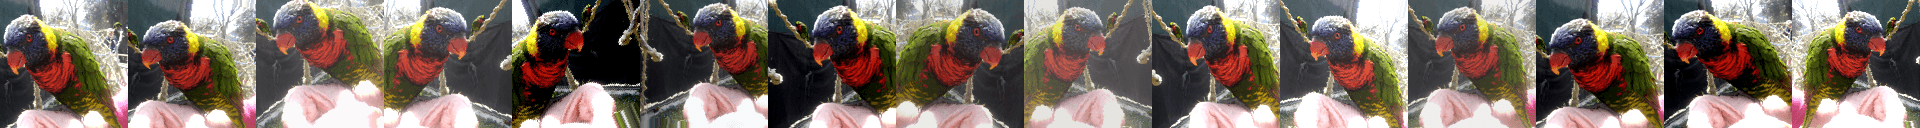
\includegraphics[width = \linewidth]{\imgpath/imagenet15.png}
  \end{center}
  \caption{Some examples of perceptually plausible image transformations applied on the same image, from ImageNet.}
\label{fig:intro-daug_imagenet}
\end{figure}

\section{Rethinking supervised learning}
\label{sec:intro-rethinking_supervised}
The re-emergence of deep learning during the last decade due to the noteworthy achievements of artificial neural networks built up a sort of philosophy that anything could be automatically learnt from data without human intervention, in contrast to the previous approach that required, indeed, a higher degree of manual design. However, this promise is misleading, since it misses the fact that the success of deep networks has been partly due to the human effort of manually labelling thousands of images and other data modalities \citep{russakovsky2015imagenet, cao2018vggface2}. As a matter of fact, the need for much data has been at the core of some strong criticisms of deep learning \citep{marcus2018critiquedl}. We argue instead that neither is deep learning some sort of exceptional solution to learn without inductive biases, nor is it a hopeless model class because it requires large data sets. On the contrary, we contend that the competitive advantage of artificial neural networks is that they are deep universal function approximators \citep{hornik1991functionapproximation} that have been proven to \textit{be able to} learn from large collections of data. While other models are known to scale poorly as the amount of training data increases, ANNs excel at fitting the training data and applying interpolation on unseen examples \citep{belkin2019biasvariance, hasson2020directfit}. This is a feature, not a bug. We will make faster progress if we exploit the advantages of deep learning, while being aware of its limitations.

Data augmentation, as we have seen, is an effective way of using this property: it generates examples in the regions of the input space where the model should learn how to interpolate. A commonly seen argument to defend that this should not be necessary and neural networks should be able to generalise from few examples is that humans and other animals learn---to categorise objects, for example---with very little supervision \citep{vinyals2016oneshot, marcus2018critiquedl, morgenstern2019oneshot, zador2019purelearning}. In this section, we will elaborate on our views on why we think this may be a misconception that can lead us astray and how we can benefit from rethinking the notions of supervised and unsupervised learning. We will do so by taking a look into learning theory, visual perception and biological vision and how these ideas relate to data augmentation and the contributions of this dissertation.

\subsection{Supervised biological learning}
The comparison between artificial intelligence---specifically artificial neural networks---and biological learning systems is intrinsic to the field, since one long-term goal of artificial intelligence is to mirror the capabilities of human intelligence. However, these capabilities are sometimes overestimated. One example is the argument that intelligence in nature evolves without supervision. In what follows, we will discuss three aspects of biological learning to argue against this view, in order to gain insights that better inform our progress in machine learning: first, we will discuss how generalisation requires exposure to relevant \textit{training data}; second, the role of evolution and brain development; third, the variety of supervised signals that the brain may use. 

First, in the argument that machine learning models should generalise from a few examples, there seems to be a promise or aspiration that with future better methods it will be possible for a neural network---for instance---to perform robust visual object categorisation among many object classes after being trained on one or a few examples per class. While we agree that a challenge for the near future is to \textit{more efficiently} learn from fewer examples, we should also remind ourselves that no machine learning algorithm can robustly learn anything that cannot be inferred from the data it has been trained on. While this may seem to be against the ultimate goal of deep learning and a reason to look for radically different approaches, we should also bear in mind that learning in nature is not too different. 

Even though the human visual system is remarkably robust, its capabilities are optimised for the tasks it needs to perform and largely shaped by experience, that is the \textit{training data}---and years of evolution \citep{hasson2020directfit}, as we will discuss below. For instance, from the literature on human visual perception, we know that object recognition is viewpoint dependent \citep{tarr1998viewpointdependence}. A well-studied property of human vision is that our face recognition ability is severely impaired if faces are presented upside down \citep{yin1969invertedfaces, valentine1988invertedfaces}. Setting aside the specific complexity of face processing in the brain, a compelling explanation for this impairment is that we are simply not used to seeing and recognising inverted faces. More generally, human perception of objects and our recognition ability is greatly affected when we see objects from unfamiliar viewpoints \citep{edelman1992viewpointdependence, tarr1998viewpointdependence, bulthoff2006viewpointdependence, milivojevic2012viewpointdependence}. Furthermore, although better than the \textit{one-shot} or \textit{few-shot} generalisation of current ANNs, humans also have limited ability to recognise novel classes \citep{morgenstern2019oneshot}. Interestingly, experiments with some novel classes of objects, known as Greebles, showed that with sufficient experience and training, humans can acquire expertise in recognising new objects from different viewpoints, even making use of an area of the brain---the fusiform face area---that typically responds strongly with face stimuli \citep{gauthier1999greebles}. This provides evidence that \textit{generalisation} to multiple viewpoints is only developed after exposure to similar conditions. In this regard, data augmentation seems like a straightforward way to provide certain degree of input variability.

Second, the commonplace comparison of artificial neural networks with the brain often misses a fundamental component of biology, recently brought to the fore by \citet{zador2019purelearning} and \citet{hasson2020directfit}, although considered since the early days of artificial intelligence \citep{turing1948intelligentmachinery}: the role that millions of years of evolution have played in developing the nervous systems of organisms in nature, including the human brain. For example, some similarities have been observed between the representational geometry of the internal features learnt by ANNs trained for visual object recognition and that of the neural activations measured in the visual cortex of the brain \citep{yamins2014annsbrains, khaligh2014annbrains, gucclu2015annbrains}. These articles were followed up by numerous studies that postulate ANNs as models of the visual cortex. However, what exactly drives better similarity with the brain remains an open question and this line of research presents several challenges. 

While artificial neural networks are typically trained from scratch, from random initialisation, the neural activations are often measured in the adult brain. A reasonable approach would be to at least consider insights from developmental neuroscience and the infant brain \citep{harwerth1986criticalperiods, atkinson2002developmental, gelman2011childcategorization}. Moreover, as mentioned above, an interesting avenue is to also take into account the role of evolution. A large part of the brain connectivity is encoded genetically, and some properties of the visual cortex are known to be innate, that is without prior exposure to visual stimuli \citep{zador2019purelearning}. Since neural networks are expected to learn some of these properties through extensive training on image data sets from scratch\footnote{Some interesting and promising areas in machine learning research deviate from this standard approach. For example, transfer learning and domain adaptation study the potential of features learnt on one task to be reused in different, related tasks \citep{zhuang2019transferlearning}, and continual learning studies the ways in which machine learning models can indefinitely sustain the acquisition of new knowledge without detriment of the previously learnt tasks \citep{aljundi2019continuallearning, mundt2019continuallearning}. These approaches are inspired by biological learning or share interesting properties with it.}, part of the artificial learning process may have more to do with evolution than with the visual learning capabilities of an adult brain. This may be another reason to temper the expectations that neural networks be able to learn from a few examples, without \textit{hard-wiring} some of the innate properties of the brain \citep{lindsey2019bioconstraints, malhotra2020bioconstraints} or, alternatively, simulating part of the evolutionary process.

Third, another commonly found argument has it that children, and other animals in general, learn robust object recognition without supervision. First of all, we should recall again the role of evolution, which can be interpreted as a pre-trained model, optimised through millions of years of data with natural selection as a supervised signal \citep{zador2019purelearning}. Second, we will argue against the very claim that children learn in fully unsupervised fashion. Obviously, the kind of supervision that humans make use of is not identical to that of machine learning algorithms: we do not see a class label on top of every object we look at. However, we receive supervision from multiple sources. Even though not for every visual stimulus, children do frequently receive information about the object classes they see---parents would point at objects and name them, for instance. Furthermore, humans usually follow a guided hierarchical learning: children do not directly learn to tell apart breeds of dogs, but rather start with umbrella terms and then progressively learn down the class hierarchy \citep{bornstein2010hierarchychildren}. \citet{hasson2020directfit} mention other examples of supervision from \textit{social cues}, that is from other humans, such as learning to recognise individual faces, produce grammatical sentences, read and write; as well as from embodiment and action, such as learning to balance the body while walking or grasping objects. In all these actions, we can identify a supervised signal that surely influences learning in the brain \citep{shapiro2019embodied}.

Moreover, besides this kind of explicit supervision, the brain surely makes use of more subtle, implicit supervised signals, such as temporal stability \citep{becker1999temporalstability, wyss2003temporalstability}: The light that enters the retina is not a random signal from a sequence of rapidly changing arbitrary photos, but a highly coherent and regular flow of slowly changing stimuli, especially at the higher, semantical level \citep{kording2004complexcells}. At the very least, this is how we perceive it and if such a smooth perception is a consequence instead of a cause, then it should be, again, a by-product of a long process of evolution. In the light of these insights from evolutionary theory and the explicit and implicit supervision that drives biological learning, we argue that we should temper the claims and aspirations that artificial neural networks should learn without supervision and from very few examples. Instead, we may benefit from rethinking the concept of supervision, embrace it and try to incorporate the forms of supervision present in nature into machine learning algorithms.

\subsection{Supervised machine learning}
If we open a machine learning textbook \citep{murphy2012machinelearning, abu2012learningfromdata, goodfellow2016dlbook}, we will most surely find a taxonomy of learning algorithms with a clear distinction between \textit{supervised} and \textit{unsupervised} learning. If we take a look at the deep learning literature of the past years, we will also find abundant work on some variants \textit{in between}: semi-supervised learning, self-supervised learning, etc. However, while this taxonomy can be useful, the boundaries are certainly not clear. As a matter of fact, strictly speaking, unsupervised learning is an illusion. If we recall the \textit{no free lunch} theorem \citep{wolpert1996nofreelunch}, averaged over all possible distributions, all classification algorithms are equivalent. Therefore, we need to constrain the distributions or, in other words, introduce prior knowledge---that is \textit{supervision}. Recently, \citet{locatello2018disentanglement} obtained a similar result for the case of unsupervised learning of disentangled representations: without inductive biases for both the models and the data sets, unsupervised disentanglement learning is impossible. These results are purely theoretical and do not hold in real world applications, precisely because in practice we use multiple inductive biases, even when we do so-called unsupervised learning.  

In a strict sense, even the classical, \textit{purely} unsupervised methods, such as independent component analysis or nearest neighbours classifiers, make use of priors, such as independence or distance, respectively. Without inductive bias, learning is not possible. Consider the data points in Figure~\ref{fig:unsupervised} (middle). With no prior information, all possible point categorisations are possible and equally valid. Depending on the inductive bias used, one model may find the configuration on the left, on the right, or any other. Which one is better depends on the task.

\begin{figure}[htb]
  \centering
  \begin{subfigure}{0.32 \linewidth}
      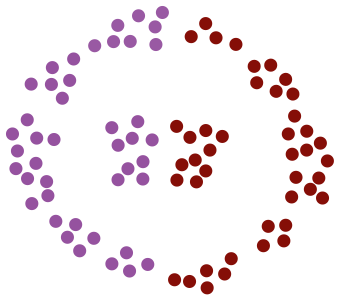
\includegraphics[keepaspectratio=true, width=\linewidth]{\imgpath/circles_lateral.png}
      \caption{One possible categorisation}
      \label{fig:lateral}
  \end{subfigure}
  \begin{subfigure}{0.32 \linewidth}
      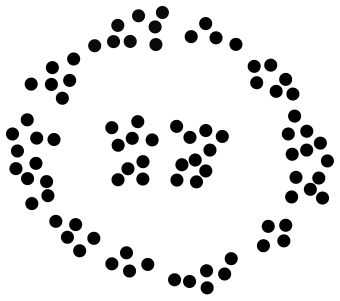
\includegraphics[keepaspectratio=true, width=\linewidth]{\imgpath/circles_all-black.png}
      \caption{A set of data points}
      \label{fig:allblack}
  \end{subfigure}
  \begin{subfigure}{0.32 \linewidth}
      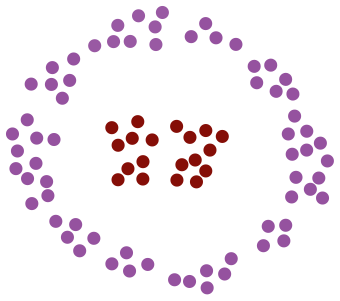
\includegraphics[keepaspectratio=true, width=\linewidth]{\imgpath/circles_concentric.png}
      \caption{One possible categorisation}
      \label{fig:concentric}
  \end{subfigure}
  \caption{An illustration of the need for inductive biases. Without any prior knowledge about the objective, any clustering of the data points is valid and can be potentially realised by a learning algorithm}
  \label{fig:unsupervised}
\end{figure}

Although this is not news, the terminology used in the machine learning literature seems to neglect these nuances and evidences that the field suffers from \textit{catastrophic forgetting}\footnote{I am borrowing the expression from Prof. Irina Rish, who used it at a panel discussion of the UNIQUE Student Symposium 2020.}. Particularly in deep learning and computer vision, the term \textit{supervised} learning is often used to actually refer to \textit{classification}, that is models trained on examples labelled according to the object classes, for instance. In turn, \textit{unsupervised} learning is used for any model that does not use the labels, regardless of what other kind of supervision may be used. Further, the term \textit{semi-supervised} learning refers to models that are trained with a fraction of the labels. While this terminology may be useful in some cases, it is not well defined and misses the fact that supervision can come in multiple flavours, not only as classification labels.

We have seen examples of different forms of supervision used by humans and other animals. What forms of supervision are common in machine learning? The relatively recent explosion of deep learning has brought about the development of several libraries for automatic differentiation\footnote{Automatic differentiation is also known as algorithmic differentiation and differentiable programming, among other names. It is the set of techniques that allows to calculate the derivatives of numeric functions algorithmically. The development of automatic differentiation libraries has played a key role in the progress of deep learning in the past 10--15 years. Examples are Theano \citep{theano2016}, TensorFlow \citep{tensorflow2015} and PyTorch \citep{pytorch2019}.} \citep{baydin2017automaticdifferentiation}, which in turn have enabled the proposal of multiple loss functions with other types of supervision that can effectively be optimised by artificial neural networks through backpropagation and stochastic gradient descent. However, these approaches are often termed in the literature \textit{semi-supervised}, \textit{self-supervised} or even \textit{unsupervised} learning. The term \textit{semi-supervised} learning has gained popularity recently \citep{jing2020selfsupervised}. On the one hand, this term acknowledges the fact that supervision is used---as opposed to unsupervised learning. On the other hand, it draws a hard line between classification and the other forms of supervised learning. The most likely reason for this separation is that labels are more costly to obtain than defining and implementing the tasks of self-supervised learning, rather than a formal, conceptual reason. From a theoretical point of view, both the conventional classification models and the recent wave of self-supervised objectives can be formalised within the category of supervised learning.

Importantly, the bulk of statistical learning theory (see a brief review in Section~\ref{sec:background-generalisation}) has been developed for binary classification loss functions, then extended for multiclass classification, and in part for regression loss functions such as the mean squared error. Critically, the mapping of many results from statistical learning theory onto the various objective functions used in semi-supervised learning is far from trivial. Given the success of this kind of supervised objectives and their connection with perception, the study of these methods from a theoretical point of view might be a fruitful direction for future work.

\section{Data augmentation, regularisation and inductive biases}
After discussing the conflict in the terminology and acknowledging that purely unsupervised learning is an illusion, we can return to the role of inductive biases from visual perception and biological vision in defining useful forms of supervision for training artificial neural networks and, in particular, the role of data augmentation. 

If we consider the particular, well-studied case of classification, to which the problem of visual object categorisation belongs, we can recall again the well-known \textit{no free lunch} theorem, which establishes that learning is not possible without any prior. The field of statistical learning theory, whose fundamental results we review in Section~\ref{sec:background-generalisation}, studies the conditions that make learning from data possible. One of its key results is that the space of possible solutions where an algorithm can search for a solution, the hypothesis set, has to be finite \citep{vapnik1971vc}. Otherwise, the problem of inferring a function from a finite set of data is ill-posed. The classical way to ensure the problem is well-posed is through regularisation \citep{phillips1962regularisation, tikhonov1963regularisation, ivanov1976regularisation}. Essentially, regularisation imposes a constraint on the hypothesis set---in the classical sense, a smoothness constraint---so that the inferred function cannot vary too rapidly around the training data points (see Section~\ref{sec:background-regularisation} for more details). Therefore, we can think of regularisation as an inductive bias. 

Being such an essential ingredient of the learning problem, regularisation has been widely studied and multiple forms of regularisation have been proposed. Two ubiquitously used regularisation techniques in deep learning are weight decay and dropout (reviewed in Section~\ref{sec:background-regularisation}). The former is a classical constraint on the norm of the learnable weights. The latter is a procedure to randomly turn off a subset of neurons during training. Both techniques have been shown to improve the generalisation of ANNs on the test data and hence their wide adoption. Thinking of regularisation techniques as inductive biases allows us to analyse the type of prior knowledge they incorporate, as well as widen the notion of regularisation to include other methods, such as data augmentation.

One of the contributions of this thesis is the comparison of weight decay, dropout and data augmentation. In Chapter~\ref{ch:daugreg}, we show that neural networks trained on image object recognition tasks \textit{without} weight decay and dropout achieve better performance than their counterparts, provided data augmentation is used during training. However, the common practice is to include all three: weight decay, dropout and data augmentation, among other methods. If we think of the inductive biases each technique introduces, data augmentation seems intuitively more advantageous: Weight decay assumes that models with smaller parameters should generalise better. Dropout assumes that neural networks that are forced to perform well with a subset of the neurons should perform better when all the neurons are used. Data augmentation makes use of an approximation of the oracle function, derived from prior knowledge about visual perception, that generates examples in regions of the input space where the model should learn a mapping. Although the inductive biases introduced by weight decay and dropout are clearly beneficial, the contribution of data augmentation seems more powerful. Nonetheless, these results were received with scepticism by the machine learning community.

In order to shed more light on the debate, we also draw theoretical insights from statistical learning theory that support the empirical findings and provide a grounded distinction between explicit regularisation methods, to which weight decay and dropout belong, and the implicit regularisation effect provided by data augmentation and other methods (Chapters~\ref{ch:reg}~and~\ref{ch:daugreg}). Explicit regularisation methods operate by directly constraining the hypothesis set of the model, known as representational capacity. However, many other methods that cannot be considered explicit regularisation provide an implicit regularisation effect, since they improve generalisation. Drawing a connection with the previously discussed ideas about supervision and inductive biases, we conclude that while explicit regularisation may indeed improve generalisation, it generally involves the optimisation of sensitive hyperparameters and at least the same or even better returns can be obtained by exploring ways of incorporating more meaningful inductive biases from visual perception and biological vision.

\section{Invariance}
In search of better inductive biases, we subscribe to the increasing trend in the machine community of exploring ways of training artificial neural networks beyond classification\footnote{Note we use the term \textit{classification}, not \textit{supervised learning}, after the discussion in Section~\ref{sec:intro-rethinking_supervised}.}. A pillar of this thesis is the attempt to integrate different disciplines. Therefore, in order to look for ways of improving visual object recognition models, we searched for inspiration in the mechanisms the brain has evolved in the visual cortex to solve object recognition.

The visual cortex is the part of the brain that processes visual information. One of its fundamental properties is the hierarchical organisation: while the primary areas of the visual cortex, which first process the information from the retina, respond to low-level properties such as the location in the visual field and the orientation of small parts of the stimuli \citep{hubelwiesel1962}, the inferior temporal (IT) cortex, later in the processing pipeline, responds to higher-level properties such as the object category of the stimulus \citep{gross1972it}. This organisation of the biological networks in the brain greatly inspired the development of artificial neural networks.

Related to the hierarchical organisation of the visual cortex, \citet{desimone1984invariantitmacaque} found that some neurons in the inferior temporal cortex of the macaque monkey responded consistently to the presentation of the same faces, regardless of their size and position. In contrast, neurons in earlier areas of the visual cortex are very sensitive to small changes in low-level properties of the visual stimuli, such as the orientation of edges. This invariance property was found to generalise to other objects besides faces \citep{booth1998invariantitmacaque} in the late 1990s and in the 2000s was observed in the human brain too \citep{quiroga2005invariantithuman}. Importantly, the invariance to identity-preserving transformations has been proposed to be an essential ingredient of robust visual object recognition in the brain \citep{dicarlo2007untangling, tacchetti2018invariance}. Hence, a reasonable question is whether artificial neural networks trained for visual object recognition are also invariant to such transformations.

The question of invariance in artificial neural networks has been addressed almost since their inception and studied from multiple perspectives. A large body of work has aimed at encoding different types of transformations into the networks (see a short review by \citet{cohen2016groupequivcnns}), such as translation or rotation invariance. One contribution of this thesis is the study of the invariance of ANNs towards identity-preserving transformations using data augmentation. The use of data augmentation is convenient: Not coincidentally, the kind of stimulus transformations tested by computational neuroscientists to study the invariance to identity-preserving transformations in the inferior temporal cortex and the image transformations typically included in data augmentation schemes are the same, or very similar. These are the transformations that we encounter naturally in the visual world, as we perceive it along the temporal dimension \citep{kording2004complexcells, einhauser2005viewpointinvariance, taylor2011temporalstability}, which perceptually preserve the object identity. For this reason we have named them \textit{perceptually plausible} transformations.

First, we measured the invariance to identity-preserving transformations of models trained on image object recognition data sets (Chapter~\ref{ch:invariance}). Intuitively and also taking the insights from the properties of the IT cortex, two images that represent different views of the same object should produce similar activations at the higher layers of a neural network. However, we found that the similarity is not better than at the pixel space, even though the models do classify the images correctly and were exposed to such transformations during training. This finding contradicts in part the general intuition that neural networks learn hierarchical representations, ranging from specific to more abstract, object-related features. We hypothesised that this is a sign of a lack of perceptual inductive bias. Given the large representational capacity of neural networks, training them with the sole objective of classifying a data set of images into the right classes does not seem enough to learn perceptually invariant representations, despite the theoretical results showing that invariance to \textit{nuisances} should emerge naturally \citep{achille2018emergence}. In general, there exist multiple possible solutions for the classification problem within the hypothesis space spanned by modern deep neural networks and the models do not seem to naturally converge to solutions well aligned with some crucial aspects of visual perception and biological vision \citep{sinz2019dlvsbrain, geirhos2020shortcutlearning, dujmovic2020adversarial}. This led us to propose \textit{data augmentation invariance}, an objective function that encourages robust representations, inspired by the invariance observed in the visual cortex.

In Chapter~\ref{ch:invariance}, we discuss the details of data augmentation invariance. We trained artificial neural networks on image object recognition data sets by jointly optimising the categorisation objective and a new data augmentation invariance objective. The latter is a layer-wise objective that encourages that the representations of transformations of the same image---generated through perceptually plausible data augmentation---cluster together. We attempted to simulate the increasing invariance along the visual cortex hierarchy by distributing the invariance loss exponentially along the neural network layers. Models trained with data augmentation invariance effectively learnt increasingly invariant representations without detriment to the classification accuracy, which even improved in some cases. 

In view of these results we argue that replacing or complementing the standard classification objectives with perceptually and biologically inspired objectives, such as data augmentation invariance, is a promising avenue to both improve computer vision algorithms and obtain better models of natural vision. Such objectives are likely not biologically plausible, in the sense that the brain does not optimise an equivalent objective \citep{pozzi2018biologicallyplausible}. However, since properties like invariance to identity-preserving transformations are at least a by-product of either evolution or early brain development (or both), it is reasonable and potentially fruitful to optimise artificial neural networks with objectives that simulate key properties of the brain.

\section{Visual salience}
So far our discussion around visual perception, biological vision and machine image understanding algorithms has revolved mainly around object recognition. However, animal vision encompasses a broader range of capabilities that allow us to navigate and understand the world. As part of the interdisciplinary pursuit of this work, we here studied some aspects of another central component of vision: visual attention.

Visual attention is a complex brain mechanism that enables us to coherently process the sheer amount of light that enters our eyes. At any given time, even though the retina receives stimulation from the whole visual field, only a small fraction of the information is processed in detail \citep{desimone1995visualattention}. Specifically, the visual system preferentially processes the information located in the centre of the visual field---the \textit{fovea}---as the central part of the retina has a larger density of photoreceptors than in the surroundings---the \textit{visual periphery} \citep{wassle1990fovea, azzopardi1993fovea}. For instance, a recent study has shown that many people fail to notice when up to 95 \% of the visual field is presented without colour \citep{cohen2020colour}. What particular area of the available information in front of us is processed in most detail at a time is mediated by eye movements, and what exactly drives eyes movement is a complex, widely studied question, which remains largely open.

For example, it is known that eye movements can be driven by both low-level properties of the stimuli---\textit{bottom-up}---and by cognitive processes derived from, for instance, a task or desire---\textit{top-down} \citep{vonstein2000topdown, munoz2004bottomup, connor2004buttomuptopdown, betz2010topdown, kollmorgen2010topdownbottomup, schutt2019bottomuptopdown}. An interesting subject of study is the relationship between object recognition and visual attention. There is strong evidence for the role of object recognition in the direction of eye movements \citep{zhaoping2007topdown}, but visual attention has been also suggested to predict object perceptual awareness \citep{holm2008attentionprecedes, kietzmann2011attentionprecedes}. 

From a behavioural perspective, the majority of the research work that studies visual attention makes use of eye tracking devices, which are able to map the gaze of an observer at any given time with the location on a stimulus. Another active area of research, at the intersection between vision science and computer vision, is the modelling of visual salience, first proposed by \citet{itti1998salience}. Salience models shift the focus to the stimulus side and aim to answer the question ``what parts of a stimulus are most salient to a human observer?''. Adhering to the definitions by \citet{kuemmerer2018salience}, a salience model predicts the probability that a pixel on a given image is fixated, which can be expressed through salience maps that represent the distribution of salience for specific tasks. For this thesis we made use of both eye tracking and salience maps to study some aspects of human vision.

In one project, presented in detail in Chapter~\ref{ch:globsal}, we were interested in studying the global salience of competing stimuli, that is stimuli presented side by side. The bulk of the research on computational models of visual salience addresses the question of what parts of a stimulus are more likely to attract the gaze of observers. In this case, we aimed at quantifying the salience of images as a whole, to seek answers for the questions: Are some types of images more likely to attract the gaze of observers? If so, is this global salience related to the local salience properties of the images? Do other factors, such as familiarity with one of the images, play a role in the gaze direction of observers? In order to answer these questions, we conducted eye tracking experiments in which we recorded the gaze direction of participants who were shown pairs of images side by side. We then modelled the behavioural data with a machine learning algorithm and computed the local salience properties of the images with representative salience models from the literature. As a main finding, we concluded that natural images intrinsically have a global salience that varies widely across different types of images and is independent of the local salience properties. 

In another study, we combined computational models of visual salience with brain measurements of functional magnetic resonance imaging (fMRI) to analyse properties of the human visual cortex. We followed up the work by \citet{zuiderbaan2017imageidentification}, where the authors showed that it is possible to identify which natural image was shown to a participant in the scanner from fMRI recordings. The predictions were made by comparing the brain activations elicited by each image on areas V1, V2 and V3, and a combination of a contrast map of the images with the receptive field properties of the cortical areas, obtained through the population receptive field (pRF) model \citep{dumoulin2008prf}. Here, we studied whether brain activity was better predicted by salience maps than by contrast maps, and extended the analysis to a broader range of visual cortical areas: V1, V2, V3, hV4, LO12 and V3AB \citep{wandell2007visualfield}. We studied two distinct models of visual salience, ICF and DeepGaze \citep{kuemmerer2017icfdeepgaze}, and concluded that salience is more predictive of brain activations than contrast, especially the salience model based on intensity and contrast information only (ICF), rather than on high-level features, suggesting that salience information is still present in the neural activations of the visual cortex.

\section{Overview of contributions and outline}
\label{sec:intro-contributions}
The overarching objective of this thesis is to explore and exploit the connections between deep artificial neural networks and the visual cognitive and neural sciences. We believe that all three fields can benefit from mutual collaboration and synergies.

In order to facilitate the understanding of the thesis to a broader audience and set the grounds for the discussion throughout the dissertation, Chapter~\ref{ch:background} provides an introduction to the fundamentals of both machine learning and visual object recognition in the brain, as well as other relevant concepts. This chapter serves also as a review of related scientific literature.

Then, a first block from Chapter~\ref{ch:reg} to \ref{ch:invariance}, has data augmentation as the central theme, starting from the rather machine learning-centred Chapter~\ref{ch:reg}, towards gradually incorporating aspects from visual perception and biological vision in the subsequent chapters.

Specifically, in Chapter~\ref{ch:reg}, we discuss the concepts of explicit and implicit regularisation and provide definitions of these terms that have been widely but ambiguously used in the literature. Part of this chapter is based on the publication \citep{hergar2018daugreg} and we here provide a longer discussion about the taxonomy of regularisation and examples of explicit and implicit regularisation, arguing in particular that data augmentation is not explicit regularisation, as considered before in the literature.

Chapter~\ref{ch:daugreg} is focused on the comparison of explicit regularisation techniques---weight decay and dropout---and data augmentation and much of the content has been published in several articles \citep{hergar2018daugadvantages, hergar2018daugreg, hergar2018wddropout}. We present the results of a systematic empirical evaluation, alongside some insights from statistical learning theory, to conclude that data augmentation alone can provide the same generalisation gain than combined with explicit regularisation, and is remarkably more flexible. In view of these results, we discuss the need for weight decay and dropout in deep learning and propose to rethink the status of data augmentation.

In Chapter~\ref{ch:daugit}, we compare the representations learnt by neural networks trained with data augmentation and the activations in the inferior temporal cortex of the human brain \citep{hergar2018daugit}. We found that models trained with heavier transformations learn features more aligned with the representations in the higher visual cortex.

Following up the connection between data augmentation and biological vision, in Chapter~\ref{ch:invariance}, we study one of the fundamental properties of the visual cortex: the increasing invariance along the ventral stream to identity-preserving transformations of visual objects. Using data augmentation as a framework to generate such transformations, we first show that standard artificial neural networks trained optimised for object categorisation are hardly robust in terms of representational similarity. Then, we propose \textit{data augmentation invariance} as a simple, yet effective and efficient way of learning robust features, while preserving the categorisation performance \citep{hergar2019dauginv}.

The last two chapters of the dissertation can be seen as a separate block, in which data augmentation and artificial neural networks are not the main subject, although machine learning is still used as a tool. Chapter~\ref{ch:globsal} is closer to the field of cognitive science, as we study some aspects of visual behaviour through an eye-tracking experiment \citep{hergar2019globsal}. In particular, we propose \textit{global visual salience} as a metric of the likelihood of competing natural images to attract the gaze of an observer. Chapter~\ref{ch:imageid} is closer to neuroimaging, as we compare models of image identification from brain data to study properties of the early visual cortex. Part of the results of this study were presented as a poster contribution at the Annual Meeting of the Visual Sciences Society in 2019 \citep{hergar2019imageid}, and we here extended the analysis.

We conclude the dissertation with a general discussion in Chapter~\ref{ch:discussion}, where we provide an overview of the main results, outline the connections between the different parts, discuss future lines of work and the broader potential impact of this work.

\chapterbibliography
}
